%%%%%%%%%%%%%%%%%%%%%%%%%%%%%%%%%%%%%%%%%%%%%%%%%%%%%%%%%%%%%%%%%%%%%%%%%%%%%%%
\chapter{Résumé de la thèse en Français}
\label{appendix:ap7-resume_de_la_thèse_en_français}
%%%%%%%%%%%%%%%%%%%%%%%%%%%%%%%%%%%%%%%%%%%%%%%%%%%%%%%%%%%%%%%%%%%%%%%%%%%%%%%

\begingroup
\etocsettocstyle{
  \addsec*{Contenus \\ \vspace{-0.5cm}
    \rule{\textwidth}{\tocrulewidth}
    \vspace{-1cm plus0mm minus0mm}
  }
}{
  \noindent\rule{\linewidth}{\tocrulewidth}
}
\localtoc
\endgroup


%%%%%%%%%%%%%%%%%%%%%%%%%%%%%%%%%%%%%%%%%%%%%%%%%%%%%%%%%%%%%%%%%%%%%%%%
\section{Introduction}
\label{section:ap7-introduction}
%%%%%%%%%%%%%%%%%%%%%%%%%%%%%%%%%%%%%%%%%%%%%%%%%%%%%%%%%%%%%%%%%%%%%%%%

%%%%%%%%%%%%%%%%%%%%%%%%%%%%%%%%%%%%%%%%%%%%%%%%%%%%%%%%%%%%%%%%%%%%%%%%%%%%%%%
\subsection{Contexte et Motivation}
\label{subsection:ap7-context_and_motivation}
%%%%%%%%%%%%%%%%%%%%%%%%%%%%%%%%%%%%%%%%%%%%%%%%%%%%%%%%%%%%%%%%%%%%%%%%%%%%%%%

\begin{figure}[t]
  \centering
  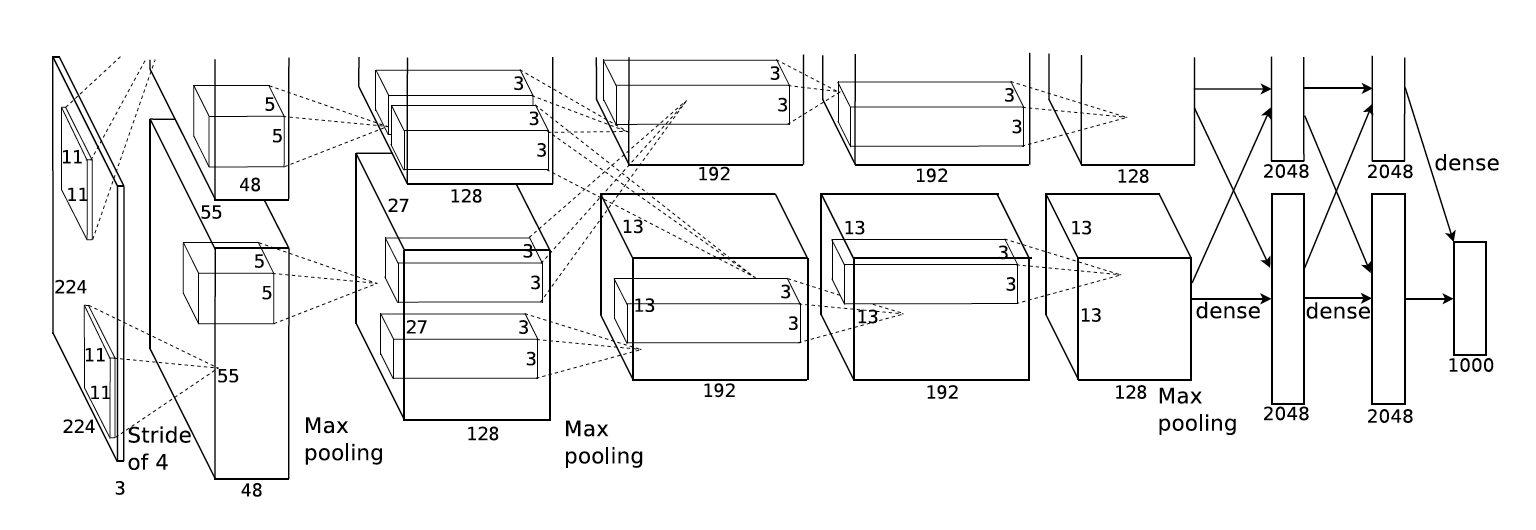
\includegraphics[scale=0.2]{figures/main/ch1-introduction/alexnet.png}
  % \caption{The neural network architecture (AlexNet) proposed by~\citet{krizhevsky2012imagenet} which won the ImageNet Large-Scale Visual Recognition Challenge in 2012.}
  \caption{L'architecture de réseau de neurones convolutifs (AlexNet), proposée par ~\citet{krizhevsky2012imagenet}, qui a remporté la compétition de reconnaissance d'image ImageNet en 2012.}
  \label{figure:ap7-alexnet_network}
\end{figure}

% One of the most remarkable breakthroughs of Deep Learning happened in 2012 during the ImageNet Large-Scale Visual Recognition Challenge~\cite{russakovsky2015imagenet}.
% The challenge aims at evaluating different algorithms for object detection and image classification.
% In 2012, \citeauthor{krizhevsky2012imagenet} obtained \nth{1} place and beat every other participant by a 10.8\% margin with a neural network architecture called \textbf{AlexNet}.
% The main reasons for this success are twofold.
% First, they used a convolutional neural network (CNN) with more than 60 million parameters which was one of the largest models of the time.
% Secondly, they designed a specific architecture to exploit dual programmable graphics processing units (GPUs) to speed up the arithmetic operations, which enabled them to significantly reduce training time.
% The \Cref{figure:ap7-alexnet_network} shows the AlexNet architecture which consists of five convolution layers with two fully connected layers at the end.
% The figure also shows the distribution of the workload between the two GPUs.

L'une des percées les plus remarquables de l'apprentissage profond s'est produite en 2012 lors de la compétition de reconnaissance d'image ImageNet~\cite{russakovsky2015imagenet}.
Cette compétition vise à évaluer différents algorithmes pour la détection d'objets et la classification d'images.
En 2012, \citeauthor{krizhevsky2012imagenet} ont obtenu la première place et ont battu tous les autres participants avec une marge de plus de 10,8\% grâce à un réseau de neurones appelé AlexNet.
Les raisons principales de ce succès sont doubles.
Premièrement, ils ont utilisé un réseau de neurones convolutif (CNN) avec plus de 60 millions de paramètres, qui était l'un des plus grands modèles de l'époque.
Deuxièmement, ils ont conçu une architecture spécifique pour exploiter deux cartes graphiques en parallèle (GPU) afin d'accélérer les opérations arithmétiques, ce qui leur a permis de réduire considérablement le temps d'apprentissage du réseau.
La figure~\ref{figure:ap7-alexnet_network} montre un schéma de l'architecture d'AlexNet qui se compose de cinq couches convolutives avec deux des couches entièrement connectées à la fin.
La figure montre également la répartition de la charge de travail entre les deux GPU.



\begin{table}[t]
  \selectlanguage{french}
  \centering
  \sisetup{
    table-number-alignment = center,
    table-space-text-pre = \ \ \ ,
  }
  \begin{subfigure}[b]{\textwidth}
    \centering
    \begin{tabular}{
      L{5cm}
      L{3.5cm}
      S[table-format=3.0, table-text-alignment=left]@{\,}
      s[table-unit-alignment=left]
      c
    }
      \toprule
      \textbf{Auteurs} & \textbf{Modèles} & \multicolumn{2}{c}{\textbf{\#Params}} & \textbf{TOP-5 Préc.} \\
      \midrule
      \citet{krizhevsky2012imagenet} & AlexNet             &  61 & \si{M} & 84.7\% \\
      \citet{simonyan2014very}       & VGG                 & 144 & \si{M} & 92.0\% \\
      \citet{he2016deep}             & ResNet-152          &  60 & \si{M} & 93.8\% \\
      \citet{szegedy2017inception}   & Inception-ResNet-v2 &  56 & \si{M} & 95.1\% \\
      \citet{xie2017aggregated}      & ResNeXt-101         &  84 & \si{M} & 95.6\% \\
      \citet{hu2018squeeze}          & SENet               & 146 & \si{M} & 96.2\% \\
      \citet{real2019regularized}    & AmoebaNet-A         & 469 & \si{M} & 96.7\% \\
      \citet{huang2019gpipe}         & AmoebaNet-B         & 556 & \si{M} & 97.0\% \\
      \bottomrule
    \end{tabular}
    \caption{Modèles de reconnaissance d'images}
    \label{table:ap7-networks_parameters_cv}
  \end{subfigure}
  \par\bigskip
  \begin{subfigure}[b]{\textwidth}
    \centering
    \begin{tabular}{
      L{4.5cm}
      L{4.5cm}
      S[table-format=3.0, table-text-alignment=left]@{\,}
      s[table-unit-alignment=left]
    }
      \toprule
      \textbf{Auteurs} & \textbf{Modèles} & \multicolumn{2}{c}{\textbf{\#Params}} \\
      \midrule
      \citet{peters2018deep}         & ELMo            &  94 & \si{M} \\
      \citet{radford2018improving}   & GPT             & 110 & \si{M} \\
      \citet{devlin2019bert}         & BERT            & 340 & \si{M} \\
      \citet{yang2019xlnet}          & XLNet (Large)   & 340 & \si{M} \\
      \citet{liu2019roberta}         & RoBERTa (Large) & 355 & \si{M} \\
      \citet{radford2019language}    & GPT-2           &   1 & \si{B} \\
      \citet{shoeybi2019megatron}    & MegatronLM      &   8 & \si{B} \\
      \citet{raffel2020exploring}    & T5-11B          &  11 & \si{B} \\
      \citet{rosset2020turingnlg}    & T-NLG           &  17 & \si{B} \\
      \citet{brown2020language}      & GPT-3           & 175 & \si{B} \\
      \citet{fedus2021switch}        & Switch Transformers & 1 & \si{T} \\
      \bottomrule
    \end{tabular}
    \caption{Modèles de traitement automatique des langues}
    \label{table:ap7-networks_parameters_nlp}
  \end{subfigure}
  \par\bigskip
  % \caption{Evolution of the number of parameters for Computer Vision and Natural Language Processing models developed in the years after AlexNet.}
  \caption{Évolution du nombre de paramètres des modèles de reconnaissance d'image et de traitement du langage naturel développés dans les années qui ont suivi l'architecture AlexNet.}
  \label{table:ap7-networks_parameters}
\end{table}


% Following this result, many architectures with an increasing number of parameters have been developed.
% This growth in the number of parameters has led to an increase in accuracy, exceeding even human performance, on the ImageNet dataset~\cite{he2015delving}.
% \Cref{table:ap7-networks_parameters} shows a list of the different state-of-the-art architectures along with their size and accuracy.
% As we can see, the accuracy of the models generally improves at the cost of the model size.
% For computer vision models, \citet{tan2019efficientnet} have shown that the relationship between model size and accuracy seems to obey a power law.
% This relationship has also been observed for Natural Language Processing (NLP) neural networks \cite{rosenfeld2020a,kaplan2020scaling} aided by the availability of large-scale datasets such as the Common Crawl dataset~\cite{raffel2020exploring} which constitutes nearly a trillion words.

Après l'introduction d'AlexNet, de nombreuses architectures avec un nombre croissant de paramètres ont été développées.
Cette augmentation du nombre de paramètres a conduit à une augmentation de la précision des modèles, dépassant même les performances humaines, sur l'ensemble de données d'ImageNet~\cite{he2015delving}.
Le Tableau~\ref{table:ap7-networks_parameters} montre une liste des différentes architectures de pointe avec leur taille et leur précision.
Comme on peut le voir, la précision des modèles s'améliore généralement au prix de la taille du modèle.
Pour les modèles de vision par ordinateur, \citet{tan2019efficientnet} ont montré que la relation entre la taille du modèle et la précision semble obéir à une loi de puissance.
Cette relation a également été observée pour les réseaux neuronaux de traitement du langage naturel (NLP) \cite{rosenfeld2020a,kaplan2020scaling} aidés par la disponibilité de larges ensembles de données tels que le Common Crawl~\cite{raffel2020exploring} qui constitue près d'un trillion de mots.

% As a result of their size and improved accuracy, deep neural networks now achieve state-of-the-art performances in a variety of domains such as image recognition~\cite{lecun1998gradient,krizhevsky2012imagenet,he2016deep,tan2019efficientnet}, object detection~\cite{redmon2016you,liu2016ssd,redmon2017yolo9000}, natural language processing~\cite{merity2016pointer,vaswani2017attention,radford2019language,brown2020language}, speech recognition~\cite{hinton2012deep,abdel2014convolutional,yu2016automatic}, health care \cite{faust2018deep} etc.
% Specifically, computer vision and natural language processing models have achieved sufficient performance for being used in real-world applications such as autonomous vehicles~\cite{fagnant2015preparing,sharma2021automating}, translation~\cite{wu2016google}, vocal assistants~\cite{li2017acoustic}, etc.

Grâce à leur taille et à leur précision accrue, les réseaux de neurones profonds atteignent désormais des performances de pointe dans divers domaines tels que la reconnaissance d'images~\cite{lecun1998gradient,krizhevsky2012imagenet,he2016deep,tan2019efficientnet}, la détection d'objets~\cite{redmon2016you, liu2016ssd,redmon2017yolo9000}, le traitement du langage naturel~\cite{merity2016pointer,vaswani2017attention,radford2019language,brown2020language}, speech recognition~\cite{hinton2012deep,abdel2014convolutional,yu2016automatic}, le domaine de la santé \cite{faust2018deep} etc.
Les modèles de vision par ordinateur et de traitement du langage naturel ont atteint des performances suffisantes pour être utilisés dans des applications du monde réel telles que les véhicules autonomes~\cite{fagnant2015preparing,sharma2021automating}, la traduction~\cite{wu2016google}, les assistants vocaux~\cite{li2017acoustic}, etc.




% However, accuracy is not the only concern, when implemented in a critical decision process, neural networks need to be compact, cost-effective and secure.
% Although accurate, large neural networks often lack these properties.
% Indeed, training state-of-the-art models on computer vision or natural language processing tasks requires gigabytes of memory and can take several months to train on a single GPU~\cite{krizhevsky2012imagenet,brown2020language}.
% For example, the GPT-3 model proposed by~\citet{brown2020language}, culminates at 175 billion parameters and requires 355 years of training on a single GPU and \$\numprint{4600000} to train on a cloud-computing platform \cite{li2020overview}.
% It has also been estimated by \citet{strubell2019energy} that the training and development costs of the large Transformer model proposed by~\citet{vaswani2017attention} with neural architecture search emits an estimated \numprint{284019} kg of $\mathrm{CO}_2$ whereas a human life will consume an average of \numprint{5000} kg of $\mathrm{CO}_2$ for one year. 
% Furthermore, with the rise of smartphones and ``Internet of things'' devices (IoT) with limited computational and memory resources, neural networks also need to be efficient during the inference phase.
% In addition, with the growing concern over data privacy, methods such as \emph{federated learning} are gaining ground.
% Federated learning involves training a model across multiple decentralized devices (\eg, smartphones) with local data samples.
% This avoids the step of centralizing all users' data into one server, thus addressing the issue of data privacy.
% Thus, building compact and cost-effective neural networks have been an important goal in order to reduce training time, reduce cost and allow for faster research and development.

Cependant, la précision des modèles ne devrait pas être la seule préoccupation, lorsqu'ils sont mis en œuvre dans un processus de décision critique, les réseaux de neurones doivent être compacts, efficaces et sécurisés.
Bien que précis, les grands réseaux de neurones n'ont souvent pas ces propriétés.
En effet, l'entraînement de modèles de pointe sur des tâches de reconnaissance d'image ou de traitement du langage naturel nécessite des gigaoctets de mémoire et peut prendre plusieurs mois sur un seul GPU~\cite{krizhevsky2012imagenet,brown2020language}.
Par exemple, le modèle GPT-3 proposé par~\citet{brown2020language}, culmine à 175 milliards de paramètres et l'entraînement durerait 355 ans sur un seul GPU et coûterait \$\numprint{4600000} sur une plateforme de cloud computing \cite{li2020overview}.
Il a également été estimé par \citet{strubell2019energy} que la formation et le développement du modèle Transformer proposé par~\citet{vaswani2017attention} avec l'optimisation des hyperparamètres émettraient environ \numprint{284019} kg de $\mathrm{CO}_2$ alors qu'une vie humaine consomme en moyenne seulement \numprint{5000} kg de $\mathrm{CO}_2$ pendant un an. 
En outre, avec l'essor des smartphones et des objets connectés aux ressources de calcul et de mémoire limitées, les réseaux de neurones doivent également être efficaces pendant la phase d'inférence, c'est-à-dire, la phase d'exécution du modèle.
De plus, avec la préoccupation croissante concernant la confidentialité des données, des méthodes telles que l'``apprentissage collaboratif'' gagnent du terrain.
L'apprentissage collaboratif consiste à entraîner un modèle sur plusieurs appareils décentralisés (par exemple les smartphones) avec des échantillons de données locales.
Cela permet d'éviter l'étape de centralisation de toutes les données des utilisateurs sur un seul serveur, ce qui permet de résoudre le problème de la confidentialité des données.
Ainsi, la construction de réseaux de neurones compacts et efficaces reste un objectif important afin de réduire le temps d'entraînement, de diminuer les coûts et de permettre une R\&D plus rapide.




% In addition to being compact and cost-effective, neural networks also need to be secure.
% Due to a high complexity and expressivity, large neural networks exhibit instability to small perturbations of their inputs.
% Unstable neural networks tend to be vulnerable to \emph{adversarial examples}, \ie, imperceptible variations of natural examples, crafted to deliberately mislead the models~\cite{globerson2006nightmare,biggio2013evasion,szegedy2013intriguing}.
% The \Cref{figure:ap7-adversarial_image_example} gives an example of an adversarial attack on an image.
% The small perturbation (center) is added to the original image (left) leading to an adversarial image (right).
% This behavior can cause serious security problems when neural networks are used for critical decision-making (\eg, judicial decision, self-driving cars, etc.).

En plus d'être compacts et efficients, les réseaux de neurones doivent également être sécurisés.
En raison de leur grande complexité et expressivité, les larges réseaux de neurones sont instables aux petites perturbations.
Ainsi, cette instabilité mène à des vulnérabilités face aux \emph{exemples antagonistes}, c'est-à-dire aux variations imperceptibles des exemples naturels, conçus pour tromper délibérément les modèles~\cite{globerson2006nightmare,biggio2013evasion,szegedy2013intriguing}.
La Figure~\ref{figure:ap7-adversarial_image_example} présente un exemple antagoniste sur une image.
La petite perturbation (au centre) est ajoutée à l'image originale (à gauche), ce qui donne une image contradictoire (à droite).
Ce comportement peut causer de graves problèmes de sécurité lorsque des réseaux neuronaux sont utilisés pour des prises de décisions critiques (par exemple, les décisions judiciaires, les voitures autonomes, etc.).


% This thesis focuses on the problem of training neural networks which are not only accurate but also compact, easy to train, reliable and robust to adversarial examples.

Cette thèse se concentre sur l'entraînement de réseaux de neurones qui sont non seulement précis, mais aussi compacts, efficients, faciles à entraîner, fiables et robustes aux exemples antagonistes.




%%%%%%%%%%%%%%%%%%%%%%%%%%%%%%%%%%%%%%%%%%%%%%%%%%%%%%%%%%%%%%%%%%%%%%%%%%%%%%%
\subsection{Problématiques et Contributions}
\label{subsection:ap7-problem_statement_and_contributions}
%%%%%%%%%%%%%%%%%%%%%%%%%%%%%%%%%%%%%%%%%%%%%%%%%%%%%%%%%%%%%%%%%%%%%%%%%%%%%%%


\begin{figure}[t]
   \centering
   \begin{subfigure}[t]{0.24\textwidth}
       \centering
       \begin{equation*}
	  \leftmatrix
	    a &   &   &   \\
	      & b &   &   \\
	      &   & c &   \\
	      &   &   & d
	  \rightmatrix
       \end{equation*}
       \caption*{diagonal}
   \end{subfigure}
   \hfill
   \begin{subfigure}[t]{0.24\textwidth}
       \centering
       \begin{equation*}
	  \leftmatrix
	    a & b & c & d \\
	    e & a & b & c \\
	    f & e & a & b \\
	    g & f & e & a
	  \rightmatrix
       \end{equation*}
       \caption*{Toeplitz}
   \end{subfigure}
   \hfill
   \begin{subfigure}[t]{0.24\textwidth}
       \centering
       \begin{equation*}
	  \leftmatrix
	    ae & af & ag & ah \\
	    be & bf & bg & bh \\
	    ce & cf & cg & ch \\
	    de & df & dg & dh
	  \rightmatrix
       \end{equation*}
       \caption*{Low Rank}
   \end{subfigure}
   \hfill
   \begin{subfigure}[t]{0.24\textwidth}
       \centering
       \begin{equation*}
	  \leftmatrix
	    a & a^2 & a^3 & a^4 \\
	    b & b^2 & b^3 & b^4 \\
	    c & c^2 & c^3 & c^4 \\
	    d & d^2 & d^3 & d^4
	  \rightmatrix
       \end{equation*}
       \caption*{Vandermonde}
   \end{subfigure}
  \caption{Exemples de matrices structurées.}
  \label{figure:ap7-example_structure_matrices}
\end{figure}



% Neural networks, which find their roots in the work of \citet{mcculloch1943logical,rosenblatt1958perceptron}, can be analytically described as a composition of multi-dimensional linear functions interlaced with nonlinear functions (also called activation functions).
% More formally, a neural network is a function $N_{\Omega} : \Rbb^n \rightarrow \Rbb^m$ parameterized by a set of weights $\Omega$ of the form:
% \begin{equation} \label{equation:ap7-neural_network}
%   N_{\Omega}(\xvec) = \psi^{(\depth)} \circ \rho \circ \psi^{(\depth-1)} \cdots \circ \psi^{(2)} \circ \rho \circ \psi^{(1)} (\xvec) \enspace.
% \end{equation}
% Here, $\depth$ corresponds to the \emph{depth} of the network (\ie, the number of layers) and $\rho$ is a nonlinear function.
% Finally, each $\psi^{(i)}$ is a multi-dimensional linear function $\psi^{(i)}: \xvec \mapsto \Wmat^{(i)} \xvec + \bvec^{(i)}$ parameterized by a weight matrix $\Wmat^{(i)}$ and a bias vector $\bvec^{(i)}$ and $\Omega$ is the union of the parameters of each layer. 

Les réseaux de neurones, qui trouvent leurs racines dans les travaux de \citet{mcculloch1943logical,rosenblatt1958perceptron}, peuvent être décrits analytiquement comme une composition de fonctions linéaires entrelacées avec des fonctions non linéaires (également appelées fonctions d'activation).
Plus formellement, un réseau de neurones est une fonction $N_{\Omega} : \Rbb^n \rightarrow \Rbb^m$ paramétrée par un ensemble de poids $\Omega$ de la forme:
\begin{equation} \label{equation:ap7-neural_network}
  N_{\Omega}(\xvec) = \psi^{(\depth)} \circ \rho \circ \psi^{(\depth-1)} \cdots \circ \psi^{(2)} \circ \rho \circ \psi^{(1)} (\xvec) \enspace.
\end{equation}
Ici, $\depth$ correspond à la \emph{profondeur} du réseau (c'est-à-dire, le nombre de couches) et $\rho$ est une fonction non linéaire.
Enfin, chaque $\psi^{(i)}$ est une fonction linéaire multidimensionnelle $\psi^{(i)} : \xvec \mapsto \Wmat^{(i)} \xvec + \bvec^{(i)}$ paramétrée par une matrice de poids $\Wmat^{(i)}$ et un biais $\bvec^{(i)}$ et $\Omega$ est l'union des paramètres de chaque couche. 


% Classical neural networks typically have a large number of parameters to train.
% If they have no restrictions on the weight matrices $\Wmat^{(i)}$, the layers are said to be \emph{fully connected}.
% Typically, fully connected neural networks have a large number of parameters.
% For example, a fully connected neural network with $\depth$ layers and $n$ neurons on each layer ($\Wmat^{(i)} \in \Rbb^{n \times n}$) will have $\bigO\left(pn (n + 1)\right)$ parameters.
% Since the input and output dimensions are generally large (\eg, ImageNet has an input dimension of $224^2 \times 3$ and an output of 1000), simple fully connected neural networks with few layers accumulate over hundreds of millions of parameters.
% Generally, this type of neural network has been shown to perform poorly due to a large search space.
% Moreover, they are computationally expensive, which makes them impractical for a number of use cases (smartphones, IoT devices, etc.).
% To reduce the number of parameters on each layer, researchers have devised specific linear operations that reduce the number of parameters and have better properties for the problem at hand.

% Les réseaux de neurones classiques ont généralement un grand nombre de paramètres à entraîner.
Si les réseaux de neurones n'ont pas de restriction sur les matrices de poids $\Wmat^{(i)}$, on dit que les couches sont \emph{entièrement connectées}.
En règle générale, les réseaux de neurones entièrement connectés ont un grand nombre de paramètres.
Par exemple, un réseau de neurones entièrement connecté avec $\depth$ couches et des $n$ neurones sur chaque couche ($\Wmat^{(i)} \in \Rbb^{n \times n}$) aura $\bigO\left(pn (n + 1)\right)$ paramètres.
Comme les dimensions d'entrée et de sortie sont généralement importantes (par exemple, le jeu de données ImageNet a une dimension d'entrée de $224^2 \times 3$ et une sortie de 1000), les réseaux de neurones entièrement connectés avec peu de couches peuvent facilement accumuler des centaines de millions de paramètres.
Il a été montré que ce type de réseau est peu performant, car l'entraînement n'optimise pas suffisamment bien les paramètres en raison d'un grand espace de recherche.
En outre, l'entraînement est long et complexe, ce qui les rend peu pratiques pour un certain nombre de cas d'usage (smartphones, objets connectés, etc.).
Pour réduire le nombre de paramètres sur chaque couche, de nombreux chercheurs ont mis au point des opérations linéaires spécifiques qui réduisent le nombre de paramètres et ont de nombreuses propriétés intéressantes.



\begin{figure}[t]
  \centering
  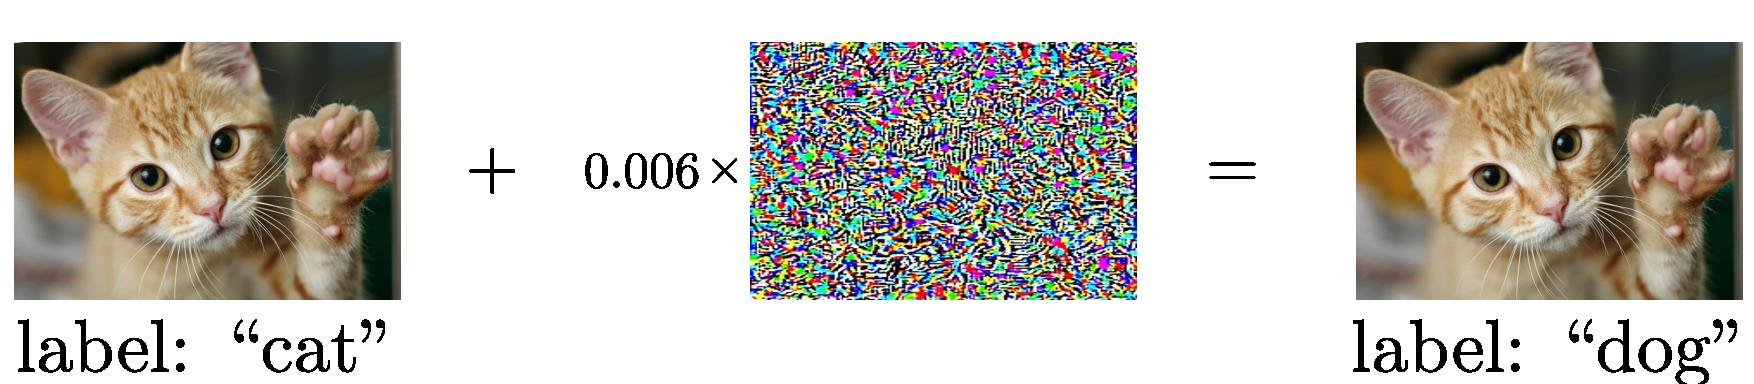
\includegraphics[width=\textwidth]{figures/main/ch1-introduction/ExampleAdversarialCatDog.pdf}
  % \caption{Example of Adversarial Attack on an image.}
  \caption{Exemple d'exemple antagoniste avec une image.}
  \label{figure:ap7-adversarial_image_example}
\end{figure}

% An example of widely used neural networks with specialized and more compact linear operations are \emph{Convolutional Neural Networks} (CNN)~\cite{lecun1998gradient,krizhevsky2012imagenet,he2016deep,tan2019efficientnet} which achieve state-of-the-art results for computer vision tasks.
% Convolutional neural networks use specific weight matrices which encode the translation invariant property often desirable to process images.
% Whereas a classical linear layer with a dense matrix will have $n \times n$ parameters, a convolution layer only has $k \times k$ parameters where $k \ll n$ is the kernel size and is usually small (\eg, 3 or 5 for classical convolution layers).
% A convolutional neural network is the most common type of \emph{structured} neural network.
% Indeed, the convolution operation can be represented by a structured matrix \ie, a matrix that can be represented with less than $n^2$ parameters.

% Un exemple de réseaux neuronaux largement utilisés avec des opérations linéaires spécialisées et plus compactes est \emph{Convolutional Neural Networks} (CNN)~\cite{lecun1998gradient,krizhevsky2012imagenet,he2016deep,tan2019efficientnet} qui obtient des résultats de pointe pour les tâches de vision par ordinateur.
Les réseaux de neurones convolutifs (CNN), qui utilisent des opérations linéaires spécialisées et plus compactes, sont considérés comme l'état de l'art concernant les tâches de vision par ordinateur~\cite{lecun1998gradient,krizhevsky2012imagenet,he2016deep,tan2019efficientnet}. 
Ces réseaux neuronaux convolutifs utilisent des matrices de poids spécifiques qui permettent une invariance du traitement par translation, ce qui est souhaitable pour traiter des images.
Alors qu'une couche linéaire classique avec une matrice dense a $n \times n$ paramètres, une couche convolutionnelle n'a que $k \times k$ paramètres avec $k$ qui correspond à la taille du noyau et qui est généralement petite (3 ou 5 pour les couches convolutionnelles classiques).
Un réseau neuronal convolutif est le type le plus courant de réseau neuronal \emph{structuré}.
En effet, l'opération de convolution peut être représentée par une matrice structurée, c'est-à-dire, une matrice qui peut être représentée avec moins de $n^2$ de paramètres.


% In addition to offering a more compact representation, the structure of certain matrices can be exploited to obtain better algorithms for the matrix-vector product, thus optimizing memory and computing operations.
% Based on the success of convolutional neural networks, researchers have studied and proposed other types of neural networks based on weight matrices with different structures~\cite{moczulski2016acdc,sindhwani2015structured}.
% \Cref{figure:ap7-example_structure_matrices} shows different types of structured matrices that have been used for deep learning.
% Although convolutional neural networks have been state-of-the-art for computer vision tasks, it remains unclear whether other types of structured neural networks can be beneficial to other types of applications and which type of structure can provide both accuracy and efficient computation.

En plus d'offrir une représentation plus compacte, la structure de certaines matrices peut être exploitée afin d'obtenir de meilleurs algorithmes pour multiplier la matrice avec un vecteur, cela permet d'optimiser la mémoire et de réduire le nombre d'opérations réalisées.
En se basant sur le succès des réseaux de neurones convolutifs, les chercheurs ont étudié et proposé d'autres types de réseaux basés sur des matrices de poids avec différentes structures~\cite{moczulski2016acdc,sindhwani2015structured}.
La Figure~\ref{figure:ap7-example_structure_matrices} montre différents types de matrices structurées qui ont été utilisées pour l'apprentissage profond.
Bien que les réseaux de neurones convolutifs soient état de l'art pour les tâches de vision par ordinateur, il reste à savoir si d'autres types de réseaux structurés pourraient être utiles à d'autres types d'applications et quel type de structure pourraient fournir à la fois précision et efficacité de calcul.


% The contributions of this thesis lie at the intersection of linear algebra, Fourier analysis and deep learning.
% As a result, we build compact and secure neural networks by leveraging the properties of structured matrices from the Toeplitz family.
% Hereafter, we detail our contributions.

Les contributions de cette thèse se situent à l'intersection de l'algèbre linéaire, l'analyse de Fourier et de l'apprentissage profond.
En conséquence, nous construisons des réseaux de neurones compacts et sécurisés en exploitant les propriétés des matrices structurées issues de la famille de Toeplitz.
Ci-après, nous détaillons nos contributions.



%%%%%%%%%%%%%%%%%%%%%%%%%%%%%%%%%%%%%%%%%%%%%%%%%%%%%%%%%%%%%%%%%%%%%%%%%%%%%%%%
\subsubsection{Entraînement de Réseaux de Neurones Compacts}
\label{subsubsection:ap7-training_compact_neural_networks}
%%%%%%%%%%%%%%%%%%%%%%%%%%%%%%%%%%%%%%%%%%%%%%%%%%%%%%%%%%%%%%%%%%%%%%%%%%%%%%%%

% As a first contribution, we use circulant matrices, which are a particular type of Toeplitz matrix, to devise a new compact architecture replacing fully connected neural networks.
% More precisely, we study deep diagonal-circulant neural networks, which are deep neural networks in which weight matrices are the product of diagonal and circulant ones.
% Besides making a theoretical analysis of their expressivity, we introduce principled techniques for training these models: we devise an initialization scheme and propose a smart use of nonlinearity functions in order to train deep diagonal-circulant networks.
% Furthermore, we show that these networks outperform recently introduced deep networks with other types of structured layers.
% We conduct a thorough experimental study to compare the performance of deep diagonal-circulant networks with state-of-the-art models. 
% We show that our models achieve better accuracy than other structured approaches while requiring 2x fewer weights than the next best approach.
% Finally, we train accurate deep diagonal-circulant networks on a real-world video classification dataset with over 3.8 million training examples.
%
% The training procedure we have developed to train large diagonal-circulant neural networks was first published in the \textbf{\color{mydarkblue} European Conference on Computer Vision Workshops on Video Classification}, as part of the \yt challenge.
% Then, the theoretical analysis of the expressivity of diagonal-circulant neural networks has been published in a second paper in the \textbf{\color{mydarkblue} 24th European Conference on Artificial Intelligence}.


% Comme première contribution, nous utilisons des matrices circulantes, qui sont un type particulier des matrices de Toeplitz, pour concevoir une nouvelle architecture de réseau de neurones compacte remplaçant les réseaux de neurones entièrement connectés.


Comme première contribution, nous étudions les réseaux de neurones dans lesquels les matrices de poids sont le produit des matrices diagonales et circulantes.
Les matrices circulantes sont un type particulier de matrice de Toeplitz.
Cette nouvelle architecture compacte permet de remplacer les réseaux de neurones entièrement connectés tout en maintenant la performance.
Outre une analyse théorique de leur expressivité, nous introduisons de nouvelles techniques pour l'entraînement de ces modèles : nous concevons une procédure d'initialisation et proposons une utilisation intelligente des fonctions de non-linéarité afin de faciliter leur entraînement.
Nous montrons que ces modèles sont plus précis que les autres approches structurées tout en nécessitant deux fois moins de poids que les meilleures approches.
Enfin, nous entraînons des réseaux de neurones profonds basés sur des matrices diagonales et circulantes sur un ensemble de données de classification vidéo qui contient plus de 3.8 millions d'exemples.

L'analyse expérimentale des réseaux de neurones profonds basée sur des matrices diagonales et circulantes sur l'ensemble de données de classification vidéo a été publiée dans le cadre de l'\textbf{\color{mydarkblue} Atelier sur la reconnaissance de vidéo de la Conférence Européenne de Vision par Ordinateur}.
Ce travail a été réalisé dans le cadre de la compétition \yt organisée par Google.
Ensuite, l'analyse théorique de l'expressivité de ces réseaux a été publiée dans un deuxième article dans le cadre de la \textbf{\color{mydarkblue} 24e Conférence Européenne sur l'Intelligence Artificielle.}



%%%%%%%%%%%%%%%%%%%%%%%%%%%%%%%%%%%%%%%%%%%%%%%%%%%%%%%%%%%%%%%%%%%%%%%%%%%%%%%%
\subsubsection{Entraînement de Réseaux de Neurones Robustes}
\label{subsubsection:ap7-training_robust_neural_networks}
%%%%%%%%%%%%%%%%%%%%%%%%%%%%%%%%%%%%%%%%%%%%%%%%%%%%%%%%%%%%%%%%%%%%%%%%%%%%%%%%

% As a second contribution, we build robust neural networks by studying the properties of the structure of convolutions.
% We devise a new upper bound on the largest singular value of convolution layers that is both tight and easy to compute.
% Our work is based on the result of~\citet{gray2006toeplitz} which states that an upper bound on the singular value of Toeplitz matrices can be computed from the inverse Fourier transform of the characteristic sequence of these matrices.
% From our analysis immediately follows an algorithm for bounding the Lipschitz constant of a convolution layer, and by extension the Lipschitz constant of the whole network.
% Finally, we illustrate our approach to adversarial robustness.
% Recent work has shown that empirical methods such as adversarial training offer poor generalization~\cite{schmidt2018adversarially} and can be improved by applying Lipschitz regularization~\cite{farnia2018generalizable}.
% To illustrate the benefit of our new method, we train neural networks with Lipschitz regularization and show that it offers a significant improvement over adversarial training alone.
%
% The main result of the work described in \Cref{chapter:ch5-lipschitz_bound} has been published in the \textbf{\color{mydarkblue}\nth{35} AAAI Conference on Artificial Intelligence}.
% Additional joint contributions have also been published on the topic of robust neural networks.
% The first work, published in the \textbf{\color{mydarkblue} Advances in Neural Information Processing Systems}, studies the effectiveness of noise injection at training and inference time in the network to protect against adversarial attacks.
% In this work, we show that noise drawn from the Exponential family offers a provable protection against adversarial attacks. 
% The second joint contribution, published in the \textbf{\color{mydarkblue} European Conference on Machine Learning Workshop for CyberSecurity}, conducts a geometrical analysis of defense mechanisms designed to protect neural networks against.
% This work shows that neural networks designed to be robust against one type of adversarial example offer poor against other types of attacks.


Comme deuxième contribution, nous proposons une procédure pour entraîner des réseaux de neurones robustes en étudiant les propriétés de la structure des convolutions.
Nous concevons une nouvelle borne supérieure des valeurs singulières des couches de convolution, qui est à la fois précise et facile à calculer.
Notre travail est basé sur le résultat de~\citet{gray2006toeplitz} qui indique qu'une borne supérieure des valeurs singulières des matrices de Toeplitz peut être calculée à partir de la transformée de Fourier inverse de la séquence caractéristique de ces matrices.
De notre analyse découle immédiatement un algorithme de régularisation de la constante de Lipschitz d'une couche convolutive, et par extension de la constante de Lipschitz de l'ensemble du réseau.
Enfin, nous utilisons notre approche pour améliorer la robustesse des réseaux de neurones convolutifs.
Des travaux récents ont montré que les méthodes empiriques telles que l'entraînement contradictoire offrent une faible généralisation~\cite{schmidt2018adversarially} et peuvent être améliorées en appliquant une régularisation Lipschitz~\cite{farnia2018generalizable}.
Pour illustrer l'avantage de notre nouvelle méthode, nous entraînons des réseaux de neurones avec la régularisation Lipschitz et montrons qu'elle offre une amélioration significative de robustesse.

Le principal résultat des travaux décrits dans le Chapitre~\ref{chapter:ch5-lipschitz_bound} a été publié dans le cadre de la  \textbf{\color{mydarkblue}35e Conférence AAAI sur l'Intelligence Artificielle}.
D'autres contributions conjointes ont également été publiées sur le thème des réseaux neuronaux robustes.
La première, publiée dans le cadre de la \textbf{\color{mydarkblue} Conférence en Intelligence Artificielle et Neurosciences Computationnelles}, étudie l'efficacité de l'injection de bruit à l'entraînement et à l'inférence dans le réseau pour protéger contre les attaques adverses.
Dans ce travail, nous montrons que le bruit tiré de la famille exponentielle offre une protection garantie contre les attaques adverses. 
La deuxième contribution conjointe, publiée dans le cadre de l'\textbf{\color{mydarkblue} Atelier de Cybersécurité de la Conférence Européenne de l'Apprentissage Automatique}, effectue une analyse géométrique des mécanismes de défense destinés à protéger les réseaux neuronaux contre différents types d'attaques.
Ce travail montre que les réseaux neuronaux conçus pour être robustes contre un type d'attaque adverse offrent peu de protection contre d'autres types d'attaques.




%%%%%%%%%%%%%%%%%%%%%%%%%%%%%%%%%%%%%%%%%%%%%%%%%%%%%%%%%%%%%%%%%%%%%%%%%%%%%%%
\section{Réseaux de Neurones Compacts basés sur les matrices Diagonales et Circulantes}
\label{section:ap7-diagonal_circulant_neural_network}
%%%%%%%%%%%%%%%%%%%%%%%%%%%%%%%%%%%%%%%%%%%%%%%%%%%%%%%%%%%%%%%%%%%%%%%%%%%%%%%


% In recent years, designing compact and accurate neural networks with a small number of trainable parameters has been an active research topic.
% It is motivated by practical applications in embedded systems (to reduce memory footprint \cite{sainath2015convolutional}), federated and distributed learning (to reduce communication \cite{konecny2016federated}), etc.
% Besides a number of practical applications, it is also an important research question whether or not models really need to be this large or if smaller networks can achieve similar accuracy~\cite{ba2014deep}.
%
% Structured matrices are at the very core of most of the work on compact networks.
% In these models, dense weight matrices are replaced by matrices with a prescribed structure (\eg, low rank matrices, Toeplitz matrices, circulant matrices, LDR, etc.).
% Despite substantial efforts  (\eg, \citet{cheng2015exploration,moczulski2016acdc}), the performance of compact models is still far from achieving an acceptable accuracy motivating their use in real-world scenarios.
% This raises several questions about the effectiveness of such models and about our ability to train them.
% In particular two main questions call for investigation:
% \begin{enumerate}
%     \item \emph{What is the expressive power of structured layers compared to dense layers?}
%     \item \emph{How to efficiently train deep neural networks with a large number of structured layers?}
% \end{enumerate}
% In this chapter we aim at answering these questions by studying deep diagonal-circulant neural networks (\aka DCNNs), which are deep neural networks in which weight matrices are the product of diagonal and circulant ones.
% The idea of using diagonal and circulant matrices together comes from a series of results in linear algebra by~\citet{muller1998algorithmic} and~\citet{huhtanen2015factoring}.
%
% To answer the first question, we propose an analysis of the expressivity of DCNNs by extending the results obtained by~\citet{huhtanen2015factoring} which states that any matrix can be decomposed into the product of $2n-1$ alternating diagonal and circulant matrices.
% We introduce a new bound on the number of diagonal-circulant products required to approximate a matrix that depends on its rank.
% Building on this result, we demonstrate that a DCNN with bounded width and small depth can approximate any dense neural networks with ReLU activations. 
%
% To answer the second question, we first describe a theoretically sound initialization procedure for DCNN which allows the signal to propagate through the network without vanishing or exploding.
% Furthermore, we provide a number of empirical insights to explain the behavior of DCNNs and show the impact on the number of nonlinearities in the network on the convergence rate and the accuracy of the network. 
% By combining all these insights, we are able (for the first time) to train large and deep DCNNs and demonstrate the good performance of these networks on a large-scale application (the \yt video classification problem) and obtain very competitive accuracy. 


Ces dernières années, la conception de réseaux neuronaux compacts et performants a été un sujet de recherche actif.
Ce domaine est motivé par des applications pratiques dans les systèmes embarqués (pour réduire l'empreinte mémoire \cite{sainath2015convolutional}), l'apprentissage fédéré et distribué (pour réduire la communication \cite{konecny2016federated}), etc.
Outre un certain nombre d'applications pratiques, la question de savoir si les modèles doivent réellement être aussi larges ou si des réseaux plus petits peuvent atteindre une précision similaire est également une question de recherche importante.

Les matrices structurées sont au cœur même de la plupart des travaux sur les réseaux compacts.
Dans ces modèles, les matrices de poids dense sont remplacées par des matrices ayant une structure précise (par exemple, les matrices de rang faible, les matrices de Toeplitz, les matrices circulantes, LDR, etc.)
Malgré des efforts importants (\citet{cheng2015exploration,moczulski2016acdc}), les performances des modèles compacts sont encore loin d'atteindre une précision acceptable motivant leur utilisation dans des scénarios du monde réel.
Cela soulève plusieurs questions sur l'efficacité de ces modèles et sur notre capacité à les entraîner.
En particulier, deux questions principales appellent à investigation :
\begin{enumerate}[leftmargin=0.5cm]
  \item Quelle est l'expressivité des couches structurées par rapport aux couches denses ?
  \item Comment entraîner efficacement des réseaux neuronaux profonds avec un grand nombre de couches structurées ?
\end{enumerate}
Dans cette thèse, nous nous efforçons de répondre à ces questions en étudiant les réseaux neuronaux basés sur les matrices diagonales et circulantes (\aka DCNN), qui sont des réseaux neuronaux profonds dans lesquels les matrices de poids sont le produit des matrices diagonales et circulantes.
L'idée d'utiliser ensemble des matrices diagonales et circulantes vient d'une série de résultats en algèbre linéaire par~\citet{muller1998algorithmic} et~\citet{huhtanen2015factoring}.

Pour répondre à la première question, nous proposons une analyse de l'expressivité des DCNN en étendant les résultats obtenus par~\citet{huhtanen2015factoring} qui indique que toute matrice peut être décomposée en un produit de $2n-1$ matrices diagonales et circulantes.
Nous introduisons une nouvelle borne sur le nombre de produits requis pour approcher une matrice qui dépend de son rang.
Sur la base de ce résultat, nous démontrons qu'un DCNN avec une largeur limitée et une faible profondeur peut être autant expressif que n'importe quel réseau de neurones dense avec des activations ReLU. 

Pour répondre à la deuxième question, nous décrivons d'abord une procédure d'initialisation pour les DCNN qui permet au signal de se propager à travers le réseau sans disparaître ou exploser.
En outre, nous fournissons un certain nombre d'expériences pour expliquer le comportement des DCNN et montrer l'impact du nombre de non-linéarités dans le réseau sur le taux de convergence et la précision. 
En combinant toutes ces connaissances, nous sommes en mesure de former des DCNN de grande taille et de grande profondeur.
Pour finir, nous démontrons les bonnes performances de ces réseaux dans le contexte de la reconnaissance de vidéo. 




%%%%%%%%%%%%%%%%%%%%%%%%%%%%%%%%%%%%%%%%%%%%%%%%%%%%%%%%%%%%%%%%%%%%%%%%%%%%%%%
\section{Constante de Lipschitz des Couches Convolutionnelles}
\label{section:ap7-lipschitz_bound}
%%%%%%%%%%%%%%%%%%%%%%%%%%%%%%%%%%%%%%%%%%%%%%%%%%%%%%%%%%%%%%%%%%%%%%%%%%%%%%%


% The last few years have witnessed a growing interest in Lipschitz regularization of neural networks, with the aim of improving their generalization~\cite{bartlett2017spectrally}, their robustness to adversarial attacks~\cite{tsuzuku2018lipschitz, farnia2018generalizable}, or their generation abilities (\eg for GANs: \citet{miyato2018spectral,arjovsky2017wasserstein}).
% Unfortunately computing  the exact Lipschitz constant of a neural network is NP-hard~\cite{scaman2018lipschitz} and in practice, existing techniques such as~\citet{scaman2018lipschitz}, \citet{fazlyab2019efficient} or~\citet{latorre2020lipschitz} are difficult to implement for neural networks with more than one or two layers, which hinders their use in deep learning applications.
%
% To overcome this difficulty, most of the work has focused on computing the Lipschitz constant of \emph{individual layers} instead.
% The product of the Lipschitz constant of each layer is an upper-bound for the Lipschitz constant of the entire network, and it can be used as a surrogate to perform Lipschitz regularization.
% Since most common activation functions (such as ReLU) have a Lipschitz constant equal to one, the main bottleneck is to compute the Lipschitz constant of the underlying linear application which is equal to its largest singular value.
% The work in this line of research mainly relies on the celebrated iterative algorithm by~\citet{golub2000eigenvalue} used to approximate the maximum singular value of a linear function.
% Although generic and accurate, this technique is also computationally expensive, which impedes its usage in large training settings.
%
% In this chapter we introduce a new upper bound on the largest singular value of convolution layers that is both tight and easy to compute.
% Instead of using the power method to iteratively approximate this value, we rely on Toeplitz matrix theory and its links with Fourier analysis.
% Our work is based on the result of~\citet{gray2006toeplitz} which states that an upper bound on the singular value of Toeplitz matrices can be computed from the inverse Fourier transform of the characteristic sequence of these matrices.
% We first extend this result to doubly-block Toeplitz matrices (\ie, block Toeplitz matrices where each block is Toeplitz) and then to convolutional operators, which can be represented as stacked sequences of doubly-block Toeplitz matrices.
% From our analysis immediately follows an algorithm for bounding the Lipschitz constant of a convolution layer, and by extension the Lipschitz constant of the whole network.
% We theoretically study the approximation of this algorithm and show experimentally that it is more efficient and accurate than competing approaches.
%
% Finally, we illustrate our approach on adversarial robustness.
% Recent work has shown that empirical methods such as adversarial training (AT) offer poor generalization~\cite{schmidt2018adversarially}, and can be improved by applying Lipschitz regularization~\cite{farnia2018generalizable}.
% To illustrate the benefit of our new method, we train a large, state-of-the-art Wide ResNet architecture with Lipschitz regularization and show that it offers a significant improvement over adversarial training alone, and over other methods for Lipschitz regularization.
% In summary, we make the three following contributions:
% \begin{enumerate}
%   \item We devise an upper bound on the singular values of the operator matrix of convolution layers by leveraging Toeplitz matrix theory and its links with Fourier analysis.
%   \item We propose an efficient algorithm to compute this upper bound which enables its use in the context of Convolutional Neural Networks.
%   \item We use our method to regularize the Lipschitz constant of neural networks for adversarial robustness and show that it offers a significant improvement over AT alone.
% \end{enumerate}

Ces dernières années ont vu un intérêt croissant pour la régularisation Lipschitz des réseaux de neurones, dans le but d'améliorer leur généralisation~\cite{bartlett2017spectrally}, leur robustesse aux attaques adverses~\cite{tsuzuku2018lipschitz, farnia2018generalizable}, ou leurs capacités de génération (par exemple pour les GANs : \citet{miyato2018spectral,arjovsky2017wasserstein}).
Malheureusement, le calcul exact de la constante de Lipschitz d'un réseau de neurones est un problème NP-complet~\cite{scaman2018lipschitz} et en pratique, les techniques existantes telles que celles proposées par~\citet{scaman2018lipschitz}, \citet{fazlyab2019efficient} ou~\citet{latorre2020lipschitz} sont difficiles à mettre en œuvre pour les réseaux neuronaux à plus d'une ou deux couches, ce qui entrave leur utilisation dans les applications d'apprentissage profond.

Pour surmonter cette difficulté au lieu de calculer la constante globale, la plupart des travaux se sont concentrés sur le calcul de la constante de Lipschitz des \emph{couches} du réseau.
Le produit des constantes de Lipschitz de chaque couche est une borne supérieure de la constante de Lipschitz de l'ensemble du réseau, et elle peut être utilisée comme substitut pour effectuer une régularisation Lipschitz.
Comme la plupart des fonctions d'activation courantes (telles que la ReLU) ont une constante de Lipschitz égale à un, la principale difficulté consiste à calculer la constante de Lipschitz de l'application linéaire sous-jacente qui est égale à sa plus grande valeur singulière.
Les travaux dans ce domaine de recherche s'appuient principalement sur un célèbre algorithme itératif appelé \emph{méthode de la puissance itérée} \cite{golub2000eigenvalue} utilisée pour approximer la valeur singulière maximale d'une fonction linéaire.
Bien que générique et précise, cette technique est également coûteuse en termes de calcul, ce qui en empêche son utilisation pour l'entraînement de larges réseaux de neurones. 

Dans cette thèse, nous introduisons une nouvelle borne supérieure des valeurs singulières des couches de convolution, qui est à la fois précise et facile à calculer.
Au lieu d'utiliser la méthode de la puissance itérée pour approximer cette valeur, nous nous appuyons sur la théorie des matrices de Toeplitz et ses liens avec l'analyse de Fourier.
Notre travail est basé sur le résultat de~\citet{gray2006toeplitz} qui indique qu'une borne supérieure des valeurs singulières des matrices de Toeplitz peut être calculée à partir de la transformée de Fourier inverse de la séquence caractéristique de ces matrices.
Nous étendons d'abord ce résultat aux matrices de Toeplitz par blocs de Toeplitz (c'est-à-dire une matrice de Toeplitz par blocs où chaque bloc est également Toeplitz) et ensuite aux opérateurs convolutionnels.
De notre analyse découle immédiatement un algorithme de régularisation de la constante de Lipschitz d'une couche convolutive, et par extension de la constante de Lipschitz de l'ensemble du réseau.
Nous étudions théoriquement l'approximation de cet algorithme et montrons expérimentalement qu'il est plus efficace et plus précis que les approches concurrentes.

Enfin, nous illustrons notre approche sur la robustesse aux exemples antagonistes.
Des travaux récents ont montré que les méthodes empiriques, telles que la formation contradictoire (\emph{Adversarial Training} ou AT), offrent une faible généralisation~\cite{schmidt2018adversarially} et peuvent être améliorées en appliquant une régularisation Lipschitz~\cite{farnia2018generalizable}.
Pour illustrer les avantages de notre nouvelle méthode, nous entraînons un large réseau de neurones avec AT et la régularisation Lipschitz et montrons qu'elle offre une amélioration significative par rapport à un entraînement contradictoire seul et par rapport aux autres méthodes de régularisation Lipschitz.
En résumé, nous apportons les trois contributions suivantes :
\begin{enumerate}[leftmargin=0.8cm]
  \item Nous proposons une nouvelle borne supérieure des valeurs singulières des couches convolutionnelles en nous appuyant sur la théorie des matrices de Toeplitz et ses liens avec l'analyse de Fourier.
  \item Nous proposons un algorithme efficace pour calculer cette borne qui permet son utilisation dans le contexte des réseaux neuronaux convolutifs.
  \item Nous utilisons notre méthode pour régulariser la constante de Lipschitz des réseaux de neurones et montrons qu'elle permet un gain significatif de robustesse face aux attaques adverses.
\end{enumerate}







